\setchapterpreamble[u]{%
\dictum[Johann Wolfgang von Goethe]{Es ist nicht genug, zu wissen, man muß auch anwenden; es ist nicht genug, zu wollen, man muß auch tun. \dots}}
\chapter{System- und Softwareentwurf} \index{System- und Softwareentwurf}\label{kap:systemundsoftwarentwurf}


Dieses Kapitel beschreibt den System- und Softwareentwurf sowie die Auswahl der Umgebung, Plattform, Software, Programmiersprache und Frameworks.

\section{Auswahlprozess}

\subsection{WebService}
Wenn von WebServices gesprochen wird, dann werden meistens SOAP-basierte WebServices gemeint. Allerdings gibt es die sogenannten SOAP-basierten WebServices als auch die RESTful WebServices. 

\subsubsection{Definition}

\begin{quotation}
\enquote{Web services provide the means to integrate disparate systems and expose reusable business functions over HTTP. They either leverage HTTP as a simple transport over which data is carried (e.g., SOAP/WSDL services) or use it as a cimplete application protocol that defines the semantics for service behavior (e.g. RESTful services) \citep[S. 2][]{robinsonService}}	
\end{quotation}

\subsubsection{SOAP/WSDL Web service}
Frau Janssen hat in ihrer Abschlussarbeit einen Web Service nach ISO 29002-20 mittels einem SOAP/WSDL Web Service implementiert \citep[vgl.][]{janssen}. Die ISO 29002-20 verweist in Annex-B auf entsprechende WSDL-Definitionen. 
Ich möchte an dieser Stelle darauf verzichten, die Einzelheiten eines SOAP/WSDL Web Service zu erläutern und verweise auf Frau Janßens Abschlussarbeit \citep[vgl.][Kap. 3]{janssen}. 

Es sei an dieser Stelle kurz erwähnt, dass Web Services auf SOAP/WSDL basierend ein W3C\footnote{World Wide Web Consortium - http://www.w3.org} Standard sind. RESTful WebServices sind per se kein Standard sondern eher ein Programmierparadigma respektive Architekturmuster. 

\subsubsection{RESTful Web service}
XXX

\subsubsection{Fazit}
Es wurde ein RESTful Web Service ausgewählt. Die Gründe stellen sich wie folgt dar:

\begin{description}
\item[Einfache Implementierung] Da RESTful Web Services auf dem HTTP Protokoll basiert und ferner sehr gute geeignete Frameworks für Java vorhanden sind, siehe Kapitel \ref{kap:bibliotheken_und_frameworks}, stellt sich für Web Entwickler die Implementierung als einfach heraus.
\item[Payload XML] Der Payload des Anfrage Queries wird als XML angegeben (siehe \ref{fig:datenfluesse}. Als mögliche Übertragung wird email angegeben. Das bedeutet für die Anforderung, das ein Web Service  implementiert werden soll, dass die XML-Repräsentation des Queries als Payload mittels XML zu übertragen ist. Folglich könnte sowohl SOAP als auch REST benutzt werden. Voraussetzung ist eine definierten Schnittstelle, welche lediglich ein XML als Payload akzeptiert. 
\item[Kein Vorteil bei SOAP] Somit hat SOAP keinen Vorteil gegenüber REST. Der Vorteil würde darin bestehen, wenn SOAP selbst die Operationen anbietet (definiert in der WSDL). Das hat den Nachteil, dass die wohlgeformte vorgegebenen Schemata query.xsd, in der Form nicht genutzt werden können. Es muss also eine Einbindung in SOAP erfolgen. 
\item[Vorteil des Payloads] Der klare Vorteil bei der Variante eine Query XML-Datei gemäß query.xsd Schema des Standards als Payload zu versenden ist der, dass eine Validierungsprüfung der XML gegen vorhandene definierte Regeln des Schemas erfolgen kann (z.B. gültige IRDI), ferner können aus dem Schema passende Modellklassen zur Verarbeitung und Speicherung der Query-Daten in der Applikation generiert werden. Mehr Informationen in Kapitel XXX (generierung mit jax).  
\end{description}




\subsection{Plattform}
Als Laufzeitumgebung wurde der Apache Tomcat Server in der Version 7 ausgewählt. Das ist ein üblicher Web Container (Web Server), welcher mit entsprechenden Frameworks bzw. Bibliotheken sowohl SOAP als auch RESTful Web Services anbieten kann. 
XXX

\subsection{Bibilotheken und Frameworks} \index{Bibilotheken und Frameworks}\label{bibliotheken_und_frameworks}
\begin{description}

\item[Jersey] Framework zur Erstellung von RESTful Web Services \index{Jersey}
\item[JSF2.0] Komponentenbasiertes Web Framework zur Erstellung von Benutzeroberflächen
\item[Spring] Dependency Injection Framework. Bietet darüber hinaus noch weitere Komponenten an. Ausgewählt wurde unter anderem Spring JDBC und Spring Data Oracle, welche einfacheren Zugriff auf relationale Datenbanken sowie auf Prozeduren von relationalen Datenbanken ermöglicht. Mehr Details zur Implementierung in Kapitel XXX.  
    
\end{description}

XXX

\subsection{Programmiersprache}
Vorgegeben ist die Umsetzung eines Web Services. Da Web Services in fast allen aktuellen Programmiersprachen entwickelt werden können, kann prinzipiell auch jede Sprache ausgewählt werden. 
Es muss die andere technische Voraussetzung erfüllt werden, die vorhandene Oracle PLIB Datenbank abrufen zu können. 

Es wurde die Sprache Java gewählt, da diese zum einen in der aktuellen Industrie stark verbreitet  und zum anderen der Autor dieser Arbeit seit vielen Jahren damit vertraut ist. 

Ein weiterer Aspekt ist, dass Software welche mit Java entwickelt wurde im Prinzip auf jeder Plattform lauffähig ist. 

\section{Softwaredesign und Architektur}

Dieses Kapitel gibt einen Überblick über das Softwaredesign und die Architektur des Systems. 

\subsection{Bausteinsicht}
\begin{quotation}
Die Bausteinsicht bildet die Aufgaben des Systems auf Software-Bausteine oder -Komponenten ab.
 \citep[S. 98ff][]{starke}	
\end{quotation}

Es soll mit Hilfe dieser Sicht ein Überblick über den Aufbau des Systems und den Abhängigkeiten der einzelnen Komponenten geschaffen werden. Dazu wird das System im top-down Ansatz aufgezeigt und verfeinert. 

\subsubsection{Level 0 - Systemüberblick mit angrenzenden Systemen} 

\begin{figure}[htbp]
	\centering
		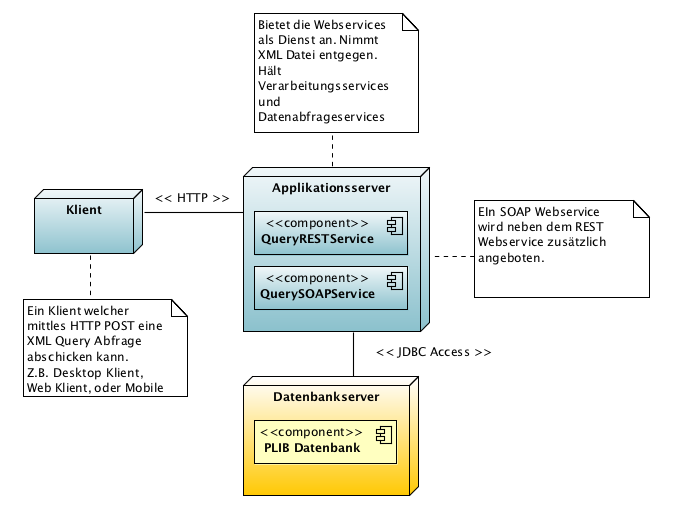
\includegraphics[width=0.9\textwidth]{images/bausteinsicht_plib_level0.png}
	\caption{Bausteinsicht Level 0}
	\label{fig:bausteinsicht_level0}
\end{figure}

\paragraph{Klient}

Der Klient stellt den Nutzer des Query Services dar. Er erzeugt das XML File, welches als Query an den Service geschickt wird. Der Transport erfolgt über das HTTP Protokoll.  

\paragraph{Applikationsserver}

Der Applikationsserver ist der Hauptbaustein. Dieser Baustein enthält alle entwickelten Komponenten. Sichtbar von außen ist der QueryService, dieser Service ist ein REST WebService und nimmt XML-Dateien als POST Request entgegen. 

\subsubsection{Level 1 - Plib characteristic query} 

Die Bausteinsicht Level 1 zeigt alle Komponenten des entwickelten Systems auf und deutet die externen Schnittstellen an. Mittels <<use>> Beziehungen erkennt man die Abhängigkeiten der einzelnen Komponenten. 

\begin{figure}[htbp]
	\centering
		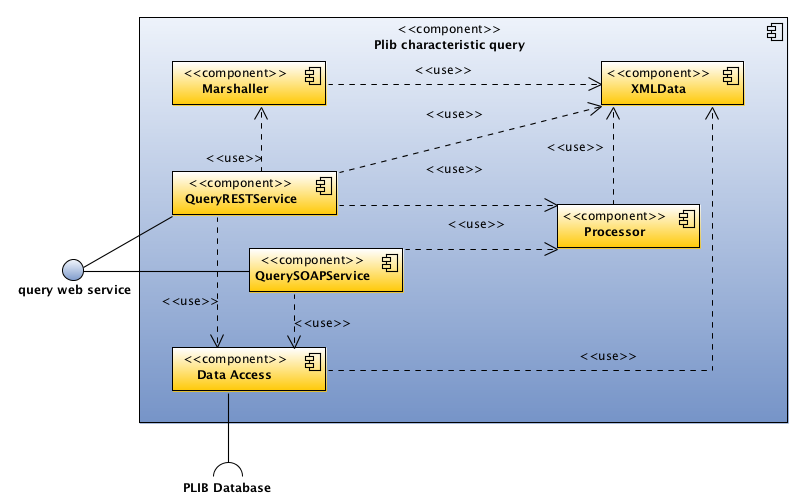
\includegraphics[width=0.98\textwidth]{images/bausteinsicht_plib_level1.png}
	\caption{Bausteinsicht - Level 1}
	\label{fig:bausteinsicht_level1}
\end{figure}

\begin{description}
\item[QueryService] Der Zweck dieser Komponente ist das entgegennehmen des Requests (Query-XML File), das Weiterleiten an die entsprechenden Weiterverarbeitenden Komponenten und letztlich das Zurücksenden der Rückantwort (Katalog-XML).
\item[Data Access] Diese technische Komponente beinhaltet die Zugriffsschicht auf die externe Datenbankschnittstelle und bietet entsprechend vereinfachte Abfrageschnittstellen für die anderen Komponenten an. 
\item[Marshaller] Eine weitere technische Komponente, diese ist für das Einlesen und Validieren der eingegangenen Query-XML Datei verantwortlich. Ferner transformiert diese Komponente die Informationen aus der Query-XML nach Validierung in das im System benutze Datenmodell aus der Komponente XMLData.
\item[XMLData] Beinhaltet das Datenmodell des Systems. Sowohl die eingehenden Query-XML Daten, als auch die ausgehenden Katalog-XML Daten werden intern in ein entsprechendes Model zur Verarbeitung abgelegt, so dass darauf gearbeitet werden kann.  
\item[Analyser] XXX
\item[Handler] XXX
\end{description}

\subsubsection{Level 2 - Whiteboxansicht - Komponente XMLData} 

Die Komponente XMLData beinhaltet alle Datenmodelle für die beiden Hauptkonzepte \enquote{Query for characteristic data} nach 

\begin{figure}[htbp]
	\centering
		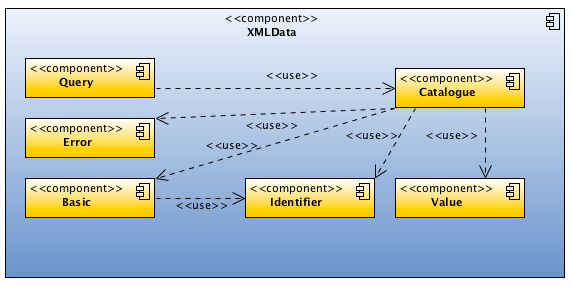
\includegraphics[width=0.82\textwidth]{images/bausteinsicht_plib_level2_xmldata.png}
	\caption{Bausteinsicht - Level 2 - Komponente XMLData}
	\label{fig:bausteinsicht_level2_xmldata}
\end{figure}

\begin{description}
\item[Query] Diese Komponente beinhaltet das Datenmodell des Queries nach ISO/TS 29002-31. 
\item[Catalogue] Diese Komponente beinhaltet das Datenmodell des Kataloges nach ISO/TS 29002-10. 
\item[Basic] Diese Komponente beinhaltet das Datenmodell von Basistypen nach ISO/TS 29002-4.
\item[Value] Diese Komponente beinhaltet das Datenmodell der Wertetypen nach ISO/TS 29002-10.
\item[Identifier] Diese Komponente beinhaltet das Datenmodell für Identifier (IRDI) nach ISO/TS 29002-5. 
\end{description}

\subsection{Klassendiagramm}

\begin{figure}[htbp]
	\centering
		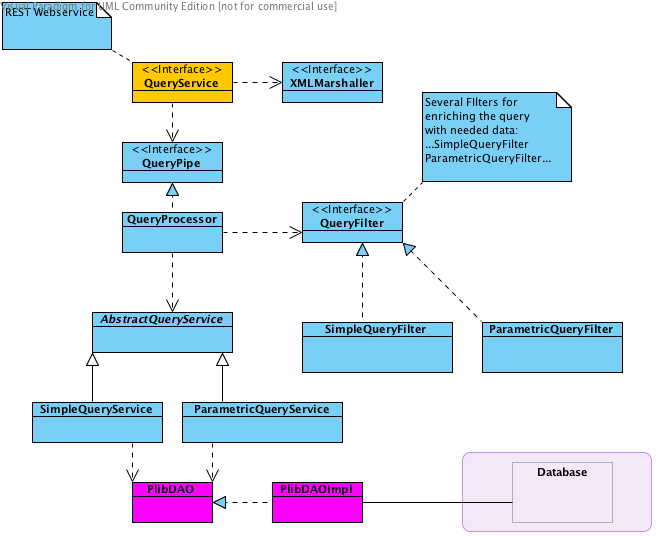
\includegraphics[width=0.98\textwidth]{images/klassendiagramm_plib.png}
	\caption{Klassendiagramm}
	\label{fig:klassendiagramm}
\end{figure}
